% ejersicios.tex
\section{Ejercicios}

\subsection{Ejercicio 1: Sistema Masa-Resorte-Amortiguador}

Resolver
\[
2\frac{d^2x}{dt^2}+8\frac{dx}{dt}+32x=0,\qquad x(0)=0{,}1\;\text{m},\quad x'(0)=0\;\text{m/s}.
\]
\textbf{Solución:} Ecuación característica $r^2+4r+16=0$ con raíces $r=-2\pm2\sqrt{3}\,i$.  
Aplicando condiciones iniciales:
\[
x(t)=e^{-2t}\left(0{,}1\cos(2\sqrt{3}\,t)+\frac{0{,}1}{\sqrt{3}}\sin(2\sqrt{3}\,t)\right).
\]
\begin{figure}[H]
\centering
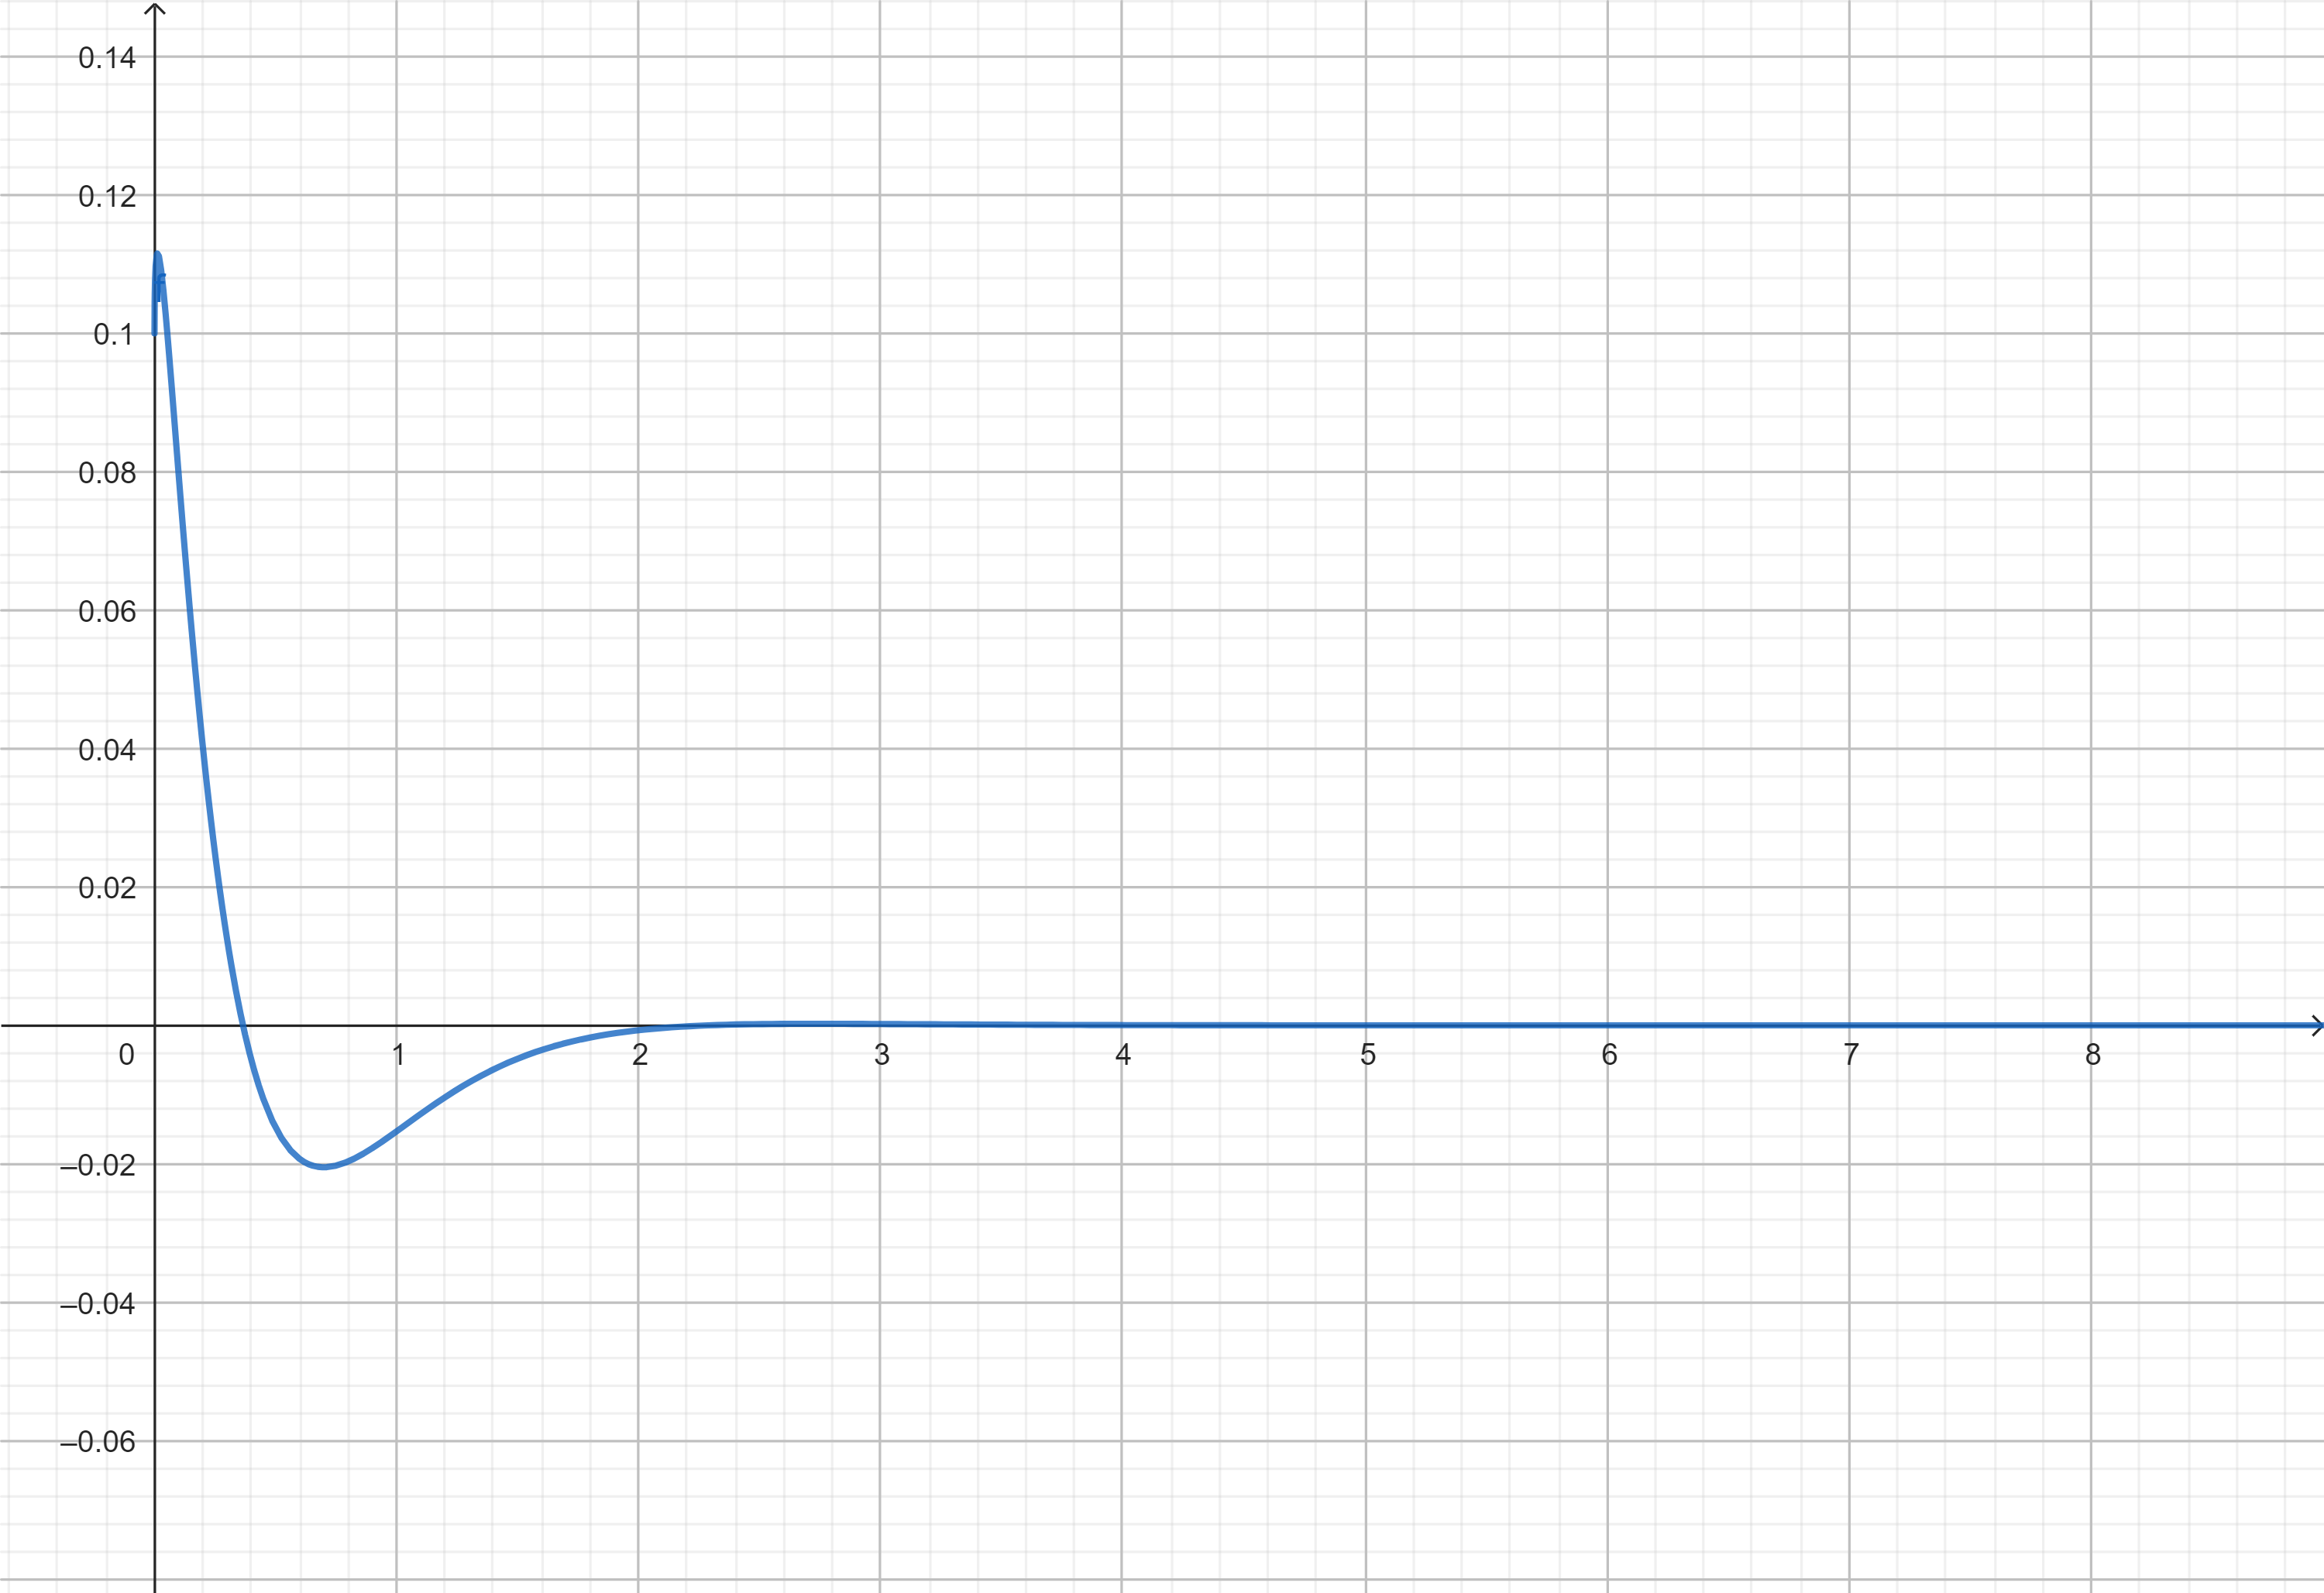
\includegraphics[width=0.8\linewidth]{imagen-ejercicio1.png}
\caption{Respuesta temporal (GeoGebra).}
\end{figure}

\subsection{Ejercicio 2: Circuito RLC en Serie}
Con $R=100\;\Omega$, $L=0{,}5$ H, $C=10\;\mu$F y condiciones iniciales $i(0)=0{,}1$ A, $i'(0)=0$, se obtiene
\[
i(t)=e^{-100t}\bigl(0{,}1\cos(400t)+0{,}025\sin(400t)\bigr).
\]
\begin{figure}[H]
\centering
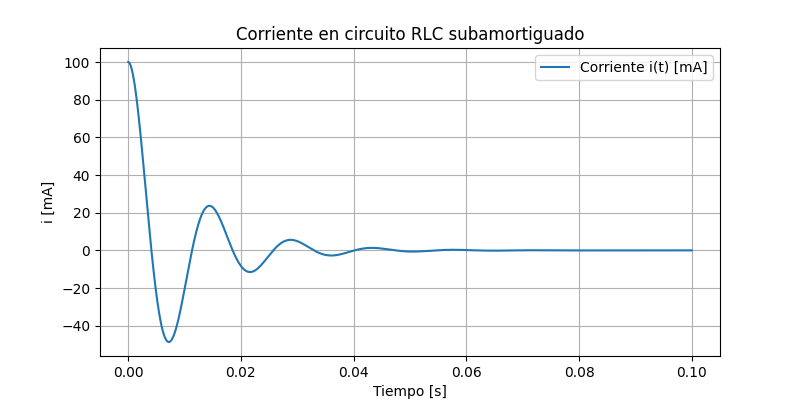
\includegraphics[width=0.8\linewidth]{imagen-ejercicio2.png}
\caption{Corriente en el circuito RLC (Python).}
\end{figure}

\subsection{Ejercicio 3: Control de Nivel}
Para $\frac{dh}{dt}+\frac{k}{A}h=0$ con $A=5$ m$^2$, $k=0{,}5$ m$^2$/s y $h(0)=2$ m:
\[
h(t)=2e^{-0{,}1t}.
\]
\begin{figure}[H]
\centering
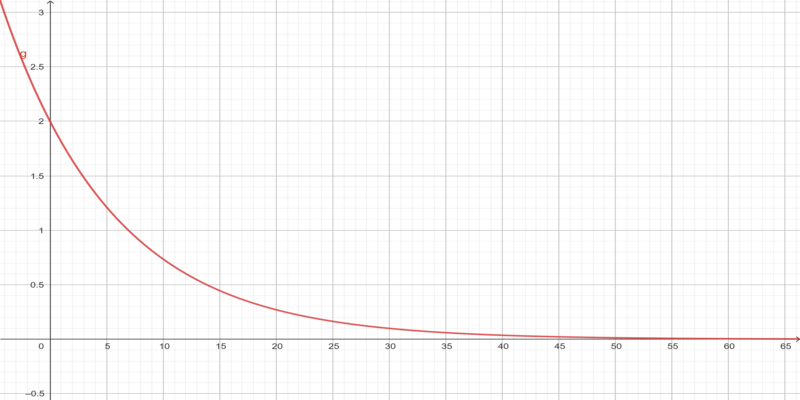
\includegraphics[width=0.8\linewidth]{imagen-ejercicio3.png}
\caption{Nivel del tanque vs.\ tiempo (GeoGebra).}
\end{figure}

\subsection{Ejercicio 4: Decaimiento de Población}
Con $\frac{dP}{dt}=-0{,}05P$ y $P(0)=100\,000$ la población se reduce a la mitad en
\[
t=\frac{\ln 0{,}5}{-0{,}05}\approx13{,}86\;\text{años}.
\]
\begin{figure}[H]
\centering
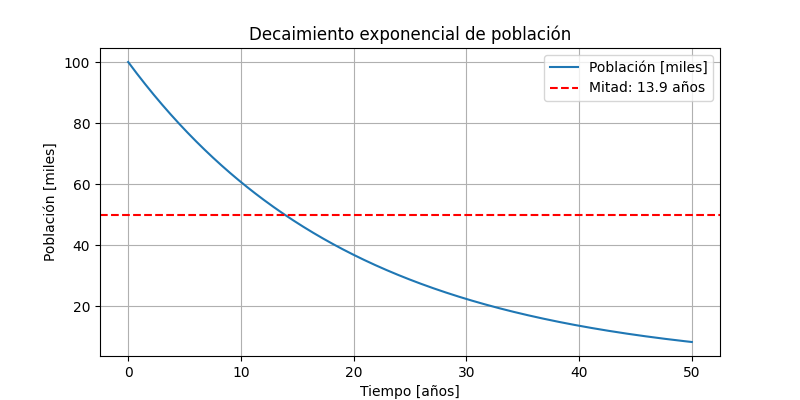
\includegraphics[width=0.8\linewidth]{imagen-ejercicio4.png}
\caption{Decaimiento exponencial (Python).}
\end{figure}

\subsection{Ejercicio 5: Sistema Sobreamortiguado}
Resolviendo
\[
\frac{d^2y}{dt^2}+6\frac{dy}{dt}+8y=0,\qquad y(0)=1,\quad y'(0)=0,
\]
se tiene $r^2+6r+8=0\Rightarrow r_1=-2,\;r_2=-4$, de donde
\[
y(t)=2e^{-2t}-e^{-4t}.
\]
\begin{figure}[H]
\centering
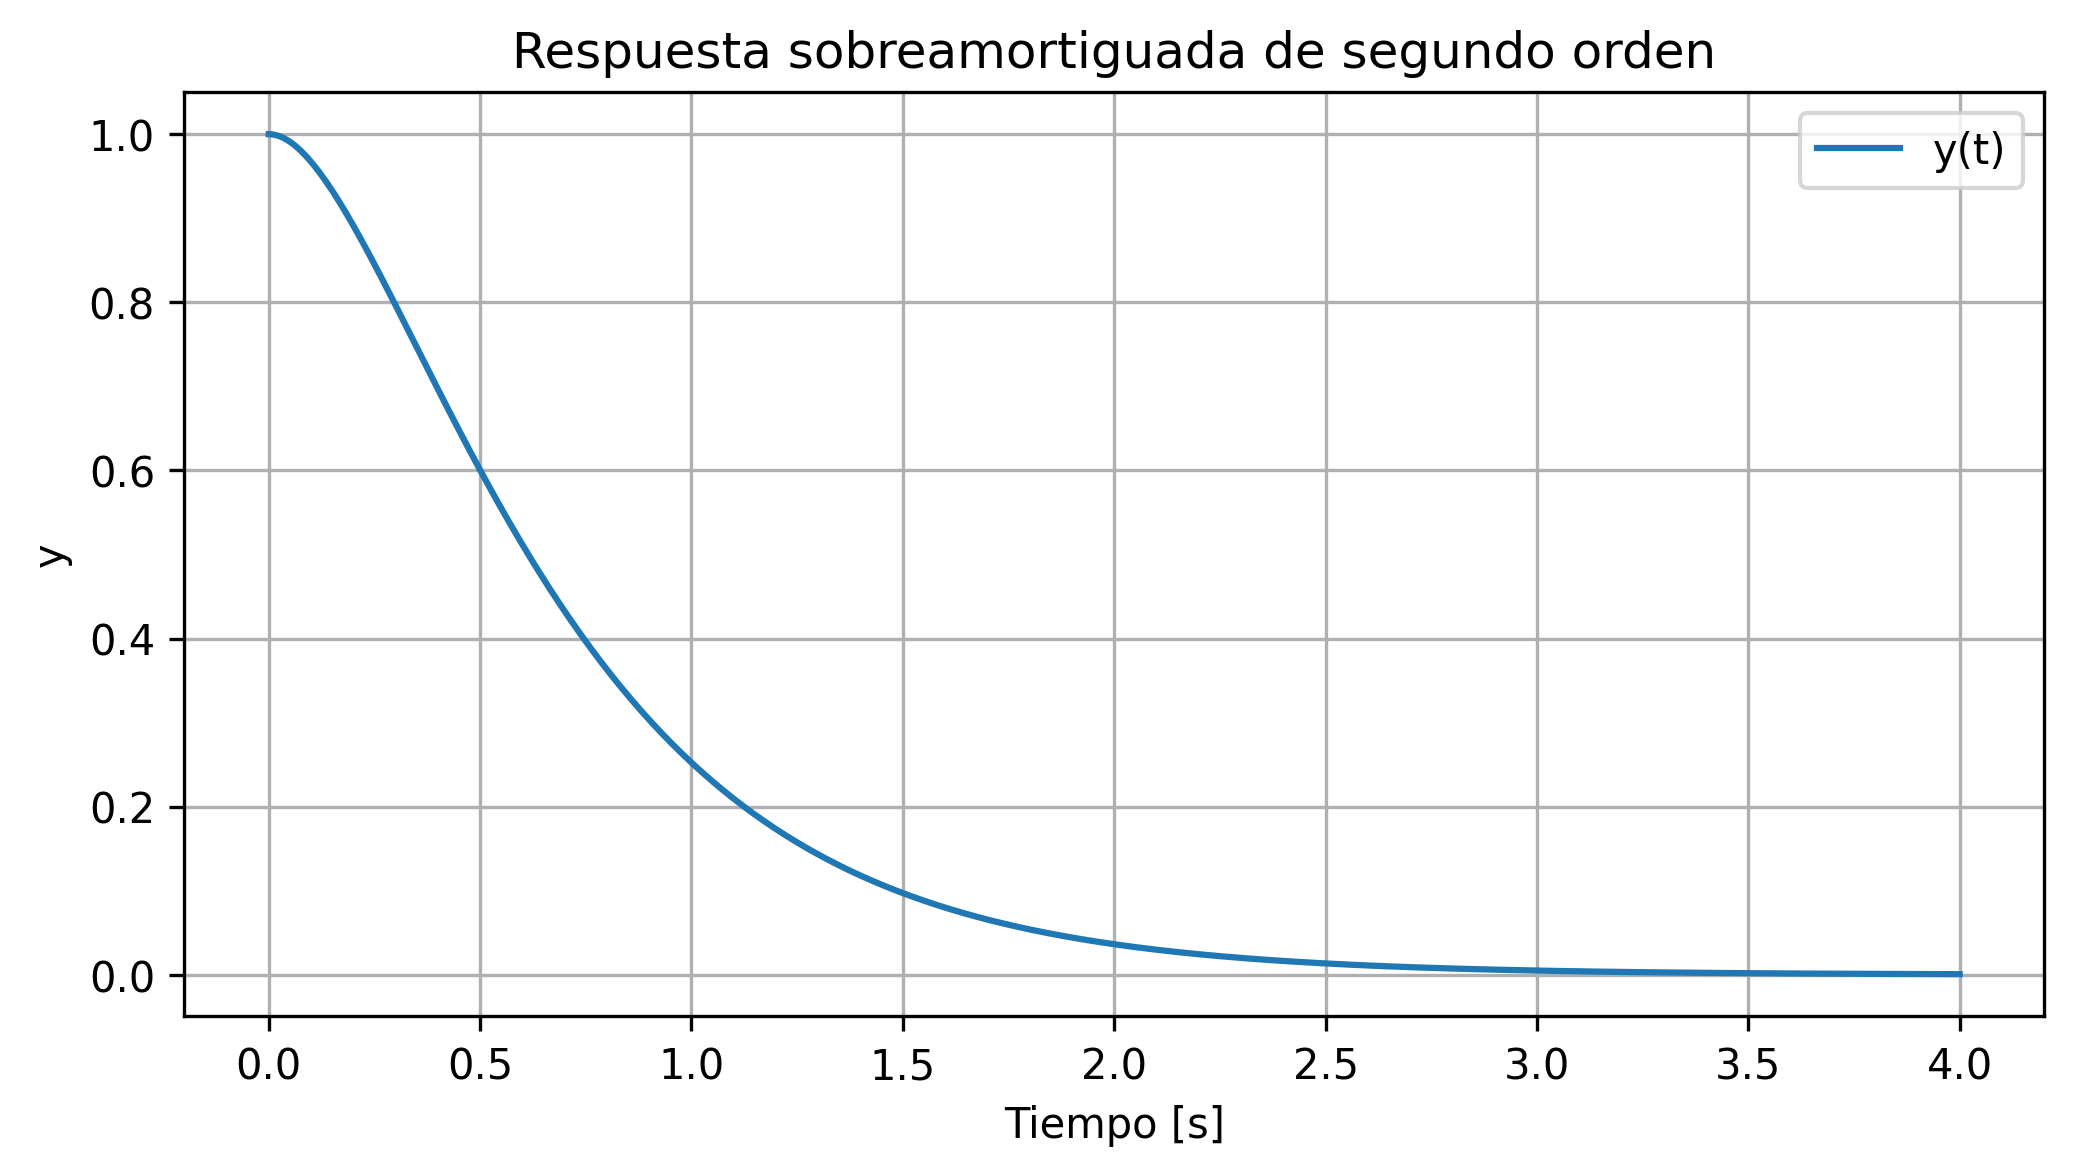
\includegraphics[width=0.8\linewidth]{imagen-ejercicio5.png}
\caption{Respuesta sobreamortiguada (GeoGebra).}
\end{figure}